\documentclass[noauthor,nooutcomes,12pt,hints]{ximera}
\graphicspath{  
{./}
{./whoAreYou/}
{./drawingWithTheTurtle/}
{./bisectionMethod/}
{./circles/}
{./anglesAndRightTriangles/}
{./lawOfSines/}
{./lawOfCosines/}
{./plotter/}
{./staircases/}
{./pitch/}
{./qualityControl/}
{./symmetry/}
{./nGonBlock/}
}


%% page layout
\usepackage[cm,headings]{fullpage}
\raggedright
\setlength\headheight{13.6pt}


%% fonts
\usepackage{euler}

\usepackage{FiraMono}
\renewcommand\familydefault{\ttdefault} 
\usepackage[defaultmathsizes]{mathastext}
\usepackage[htt]{hyphenat}

\usepackage[T1]{fontenc}
\usepackage[scaled=1]{FiraSans}

%\usepackage{wedn}
\usepackage{pbsi} %% Answer font


\usepackage{cancel} %% strike through in pitch/pitch.tex


%% \usepackage{ulem} %% 
%% \renewcommand{\ULthickness}{2pt}% changes underline thickness

\tikzset{>=stealth}

\usepackage{adjustbox}

\setcounter{titlenumber}{-1}

%% journal style
\makeatletter
\newcommand\journalstyle{%
  \def\activitystyle{activity-chapter}
  \def\maketitle{%
    \addtocounter{titlenumber}{1}%
                {\flushleft\small\sffamily\bfseries\@pretitle\par\vspace{-1.5em}}%
                {\flushleft\LARGE\sffamily\bfseries\thetitlenumber\hspace{1em}\@title \par }%
                {\vskip .6em\noindent\textit\theabstract\setcounter{question}{0}\setcounter{sectiontitlenumber}{0}}%
                    \par\vspace{2em}
                    \phantomsection\addcontentsline{toc}{section}{\thetitlenumber\hspace{1em}\textbf{\@title}}%
                     }}
\makeatother



%% thm like environments
\let\question\relax
\let\endquestion\relax

\newtheoremstyle{QuestionStyle}{\topsep}{\topsep}%%% space between body and thm
		{}                      %%% Thm body font
		{}                              %%% Indent amount (empty = no indent)
		{\bfseries}            %%% Thm head font
		{)}                              %%% Punctuation after thm head
		{ }                           %%% Space after thm head
		{\thmnumber{#2}\thmnote{ \bfseries(#3)}}%%% Thm head spec
\theoremstyle{QuestionStyle}
\newtheorem{question}{}



\let\freeResponse\relax
\let\endfreeResponse\relax

%% \newtheoremstyle{ResponseStyle}{\topsep}{\topsep}%%% space between body and thm
%% 		{\wedn\bfseries}                      %%% Thm body font
%% 		{}                              %%% Indent amount (empty = no indent)
%% 		{\wedn\bfseries}            %%% Thm head font
%% 		{}                              %%% Punctuation after thm head
%% 		{3ex}                           %%% Space after thm head
%% 		{\underline{\underline{\thmname{#1}}}}%%% Thm head spec
%% \theoremstyle{ResponseStyle}

\usepackage[tikz]{mdframed}
\mdfdefinestyle{ResponseStyle}{leftmargin=1cm,linecolor=black,roundcorner=5pt,
, font=\bsifamily,}%font=\wedn\bfseries\upshape,}


\ifhandout
\NewEnviron{freeResponse}{}
\else
%\newtheorem{freeResponse}{Response:}
\newenvironment{freeResponse}{\begin{mdframed}[style=ResponseStyle]}{\end{mdframed}}
\fi



%% attempting to automate outcomes.

%% \newwrite\outcomefile
%%   \immediate\openout\outcomefile=\jobname.oc
%% \renewcommand{\outcome}[1]{\edef\theoutcomes{\theoutcomes #1~}%
%% \immediate\write\outcomefile{\unexpanded{\outcome}{#1}}}

%% \newcommand{\outcomelist}{\begin{itemize}\theoutcomes\end{itemize}}

%% \NewEnviron{listOutcomes}{\small\sffamily
%% After answering the following questions, students should be able to:
%% \begin{itemize}
%% \BODY
%% \end{itemize}
%% }
\usepackage[tikz]{mdframed}
\mdfdefinestyle{OutcomeStyle}{leftmargin=2cm,rightmargin=2cm,linecolor=black,roundcorner=5pt,
, font=\small\sffamily,}%font=\wedn\bfseries\upshape,}
\newenvironment{listOutcomes}{\begin{mdframed}[style=OutcomeStyle]After answering the following questions, students should be able to:\begin{itemize}}{\end{itemize}\end{mdframed}}



%% my commands

\newcommand{\snap}{{\bfseries\itshape\textsf{Snap!}}}
\newcommand{\flavor}{\link[\snap]{https://snap.berkeley.edu/}}
\newcommand{\mooculus}{\textsf{\textbf{MOOC}\textnormal{\textsf{ULUS}}}}


\usepackage{tkz-euclide}
\tikzstyle geometryDiagrams=[rounded corners=.5pt,ultra thick,color=black]
\colorlet{penColor}{black} % Color of a curve in a plot



\ifhandout\newcommand{\mynewpage}{\newpage}\else\newcommand{\mynewpage}{}\fi


\title{Coloring book}
\author{Bart Snapp}

\begin{document}
\begin{abstract}
  We break symmetry by adding details.
\end{abstract}
\maketitle

\begin{listOutcomes}
\item Recognize and describe symmetry and sub-symmetries.
\item Draw pictures of given dihedral symmetries.
\item Decorate pictures so that some symmetry is broken.
\item Express rotations in terms of flips.
\end{listOutcomes}


Consider this picture:
\begin{center}
  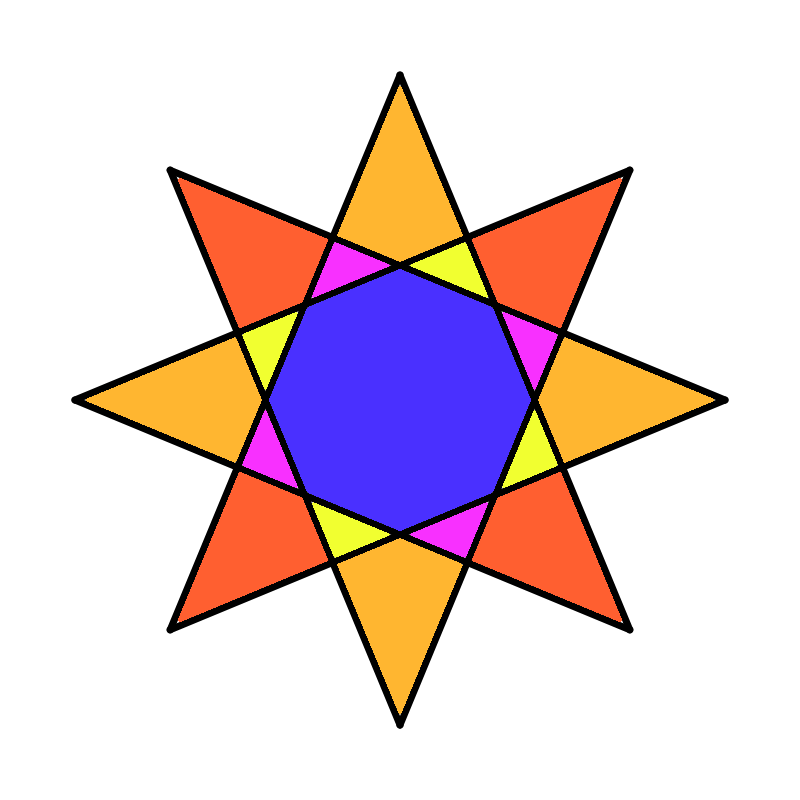
\includegraphics[width=.6\textwidth]{egR4D8.png}
\end{center}

This is a colored-in page. Setting $e$ be the do-nothing symmetry, $r$
be a clockwise $45^\circ$ rotation about the center of the hexagon,
and $f$ be a flip across a vertical line down the middle of the
picture.

BEFORE it was colored, it had $8$ rotational symmetries
\[
e,r,r^2,r^3,\dots, r^7
\]
and $8$ reflectional symmetries
\[
f,rf,r^2f, r^3f,\dots,r^7f.
\]
AFTER it was colored, it had $4$ rotational symmetries that when
EXPRESSED IN TERMS OF THE PREVIOUS SYMMETRIES we have
\[
e,r^2,r^4,r^6
\]
and NO reflectional symmetries.

\mynewpage

\begin{question}
  Consider:
  \begin{center}
    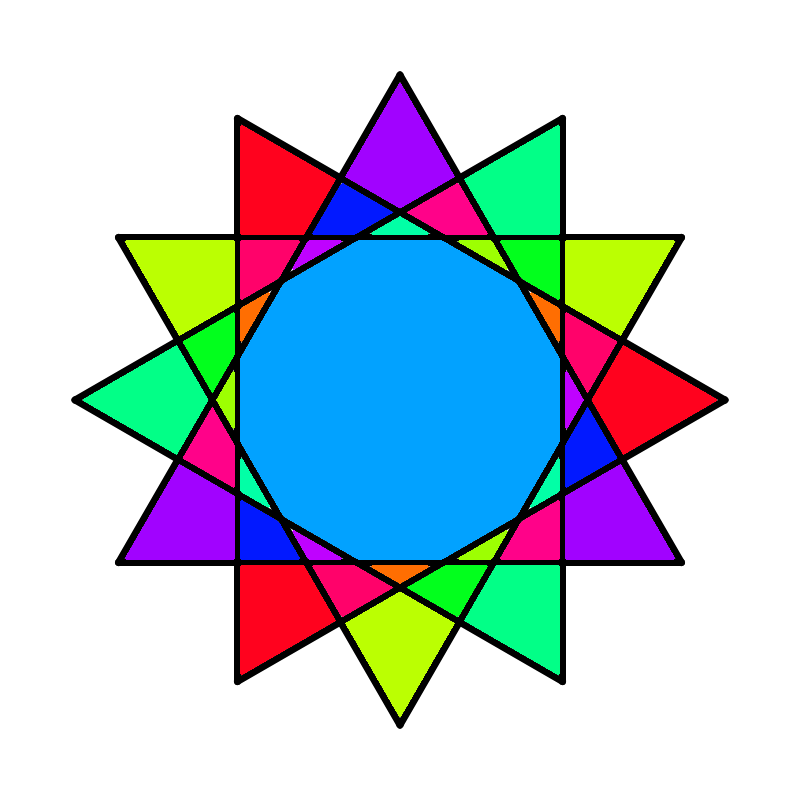
\includegraphics[width=.6\textwidth]{qR3D12.png}
  \end{center}
  \begin{enumerate}
  \item Tell me, what were the symmetries before this was colored in?
  \item Now express the symmetries of the colored-in picture in terms
    of the the symmetries of the picture BEFORE it was colored-in.
  \end{enumerate}
  \begin{freeResponse}
    \begin{enumerate}
    \item BEFORE the star was colored in, it had symmetries:
      \[
      e,r,r^2,\dots,r^{11}, f, rf,r^2f, \dots, r^{11}f
      \]
      where $r$ is a $30^\circ$ clockwise rotation, and $f$ is a flip
      across a vertical line.
    \item AFTER it is colored in, it has symmetries:
      \[
      e, r^4, r^8
      \]
      and no others.
    \end{enumerate}
  \end{freeResponse}
\end{question}
\mynewpage

\begin{question}
  Consider: 
  \begin{center}
    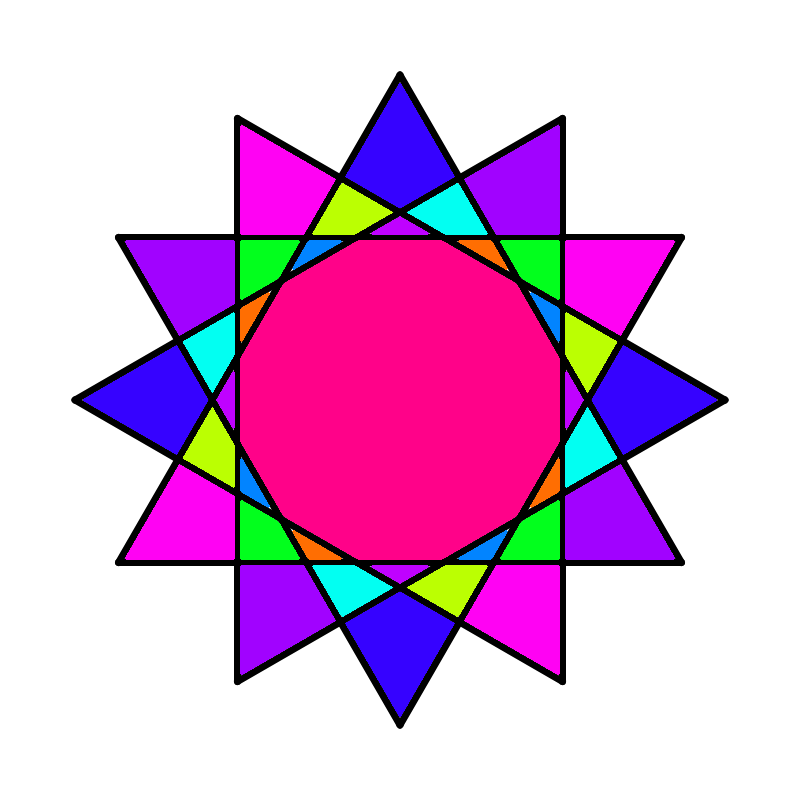
\includegraphics[width=.6\textwidth]{qR4D12.png}
  \end{center}
  \begin{enumerate}
  \item Tell me, what were the symmetries before this was colored in?
  \item Now express the symmetries of the colored-in picture in terms
    of the the symmetries of the picture BEFORE it was colored-in.
  \end{enumerate}
  \begin{freeResponse}
    \begin{enumerate}
    \item BEFORE the star was colored in, it had symmetries:
      \[
      e,r,r^2,\dots,r^{11}, f, rf,r^2f, \dots, r^{11}f
      \]
      where $r$ is a $30^\circ$ clockwise rotation, and $f$ is a flip
      across a vertical line.
    \item AFTER it is colored in, it has symmetries:
      \[
      e, r^3, r^6, r^9
      \]
      and no others.
    \end{enumerate}
  \end{freeResponse}
\end{question}
\mynewpage

\begin{question}
  Consider: 
 \begin{center}
  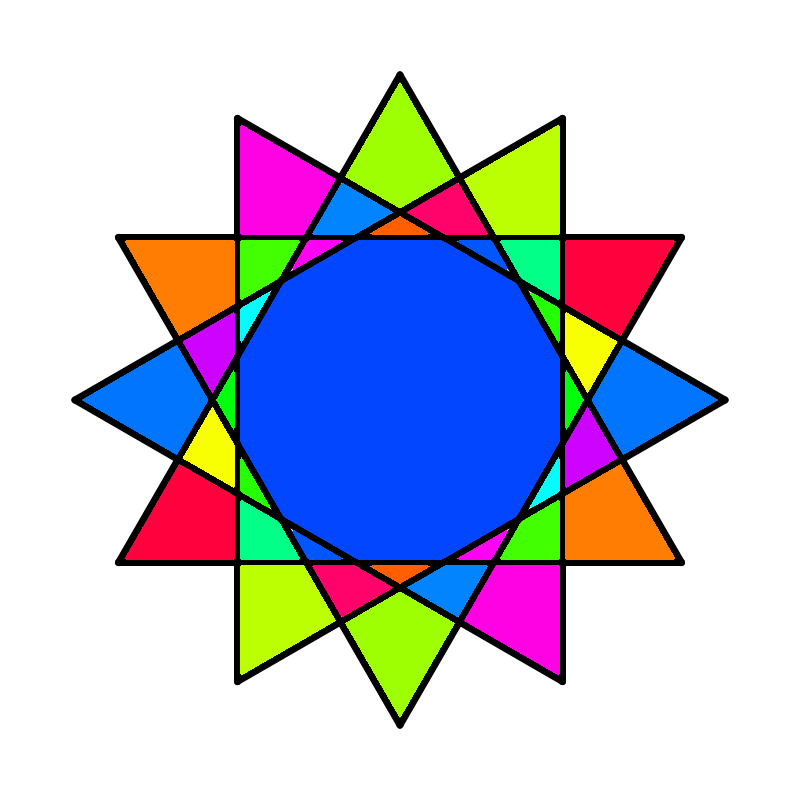
\includegraphics[width=.6\textwidth]{qR2D12.png}
 \end{center}
 \begin{enumerate}
 \item Tell me, what were the symmetries before this was colored in?
 \item Now express the symmetries of the colored-in picture in terms
    of the the symmetries of the picture BEFORE it was colored-in.
 \end{enumerate}
 \begin{freeResponse}
    \begin{enumerate}
    \item BEFORE the star was colored in, it had symmetries:
      \[
      e,r,r^2,\dots,r^{11}, f, rf,r^2f, \dots, r^{11}f
      \]
      where $r$ is a $30^\circ$ clockwise rotation, and $f$ is a flip
      across a vertical line.
    \item AFTER it is colored in, it has symmetries:
      \[
      e,r^6
      \]
      and no others.
    \end{enumerate}
  \end{freeResponse}
\end{question}
\mynewpage


\begin{question}
 Consider:
 \begin{center}
  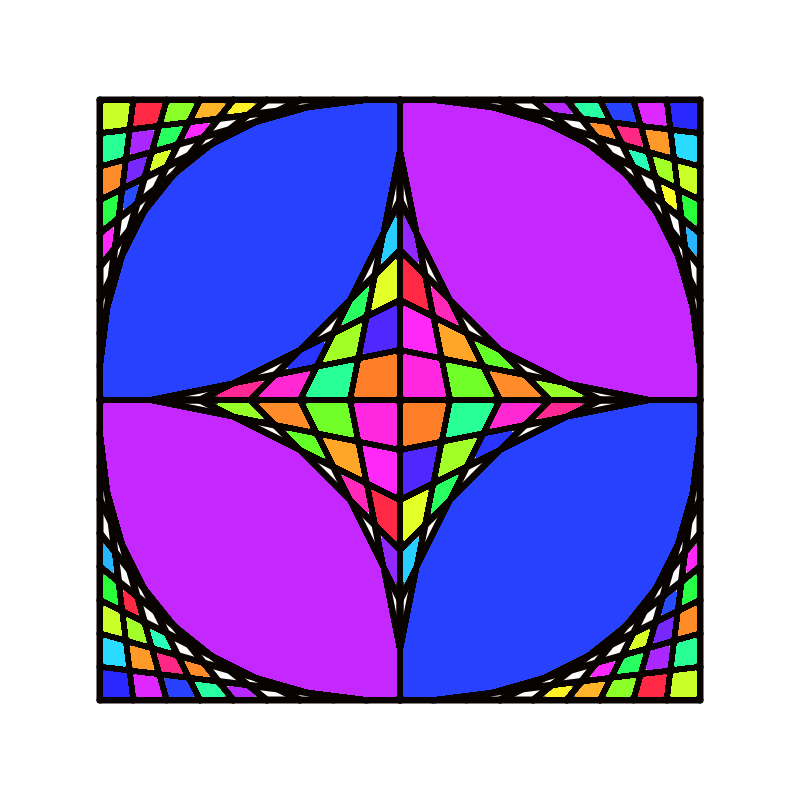
\includegraphics[width=.6\textwidth]{qR2D4.png}
 \end{center}
 \begin{enumerate}
 \item Tell me, what were the symmetries before this was colored in?
 \item Now express the symmetries of the colored-in picture in terms
    of the the symmetries of the picture BEFORE it was colored-in.
 \end{enumerate}
  \begin{freeResponse}
    \begin{enumerate}
    \item BEFORE the shape was colored in, it had symmetries:
      \[
      e,r,r^2,r^3, f, rf,r^2f,r^3f
      \]
      where $r$ is a $30^\circ$ clockwise rotation, and $f$ is a flip
      across a vertical line.
    \item AFTER it is colored in, it has symmetries:
      \[
      e,r^2
      \]
      and no others.
    \end{enumerate}
  \end{freeResponse}

\end{question}
\mynewpage

\begin{question}
  Let $r$ represent a $120$ degree clockwise rotation and $f$
  represent a flip across a vertical line through the center of the
  picture.  
 \begin{enumerate}
 \item Use an envelope of tangents to draw a picture whose symmetries
   are $e,r,r^2,f,rf,r^2f$.
 \item Now color-in your picture so that the only symmetries remaining
   are $e,r,r^2$.
 \end{enumerate}
 \begin{freeResponse}
   Here's my picture:
   \begin{center}
     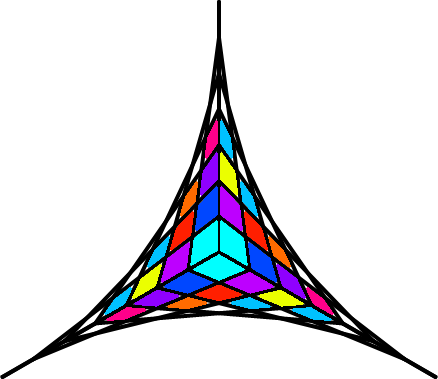
\includegraphics[width=.6\textwidth]{ansR3.png}
   \end{center}
 \end{freeResponse}
\end{question}
\mynewpage



\begin{question}
  Consider:
   \begin{center}
  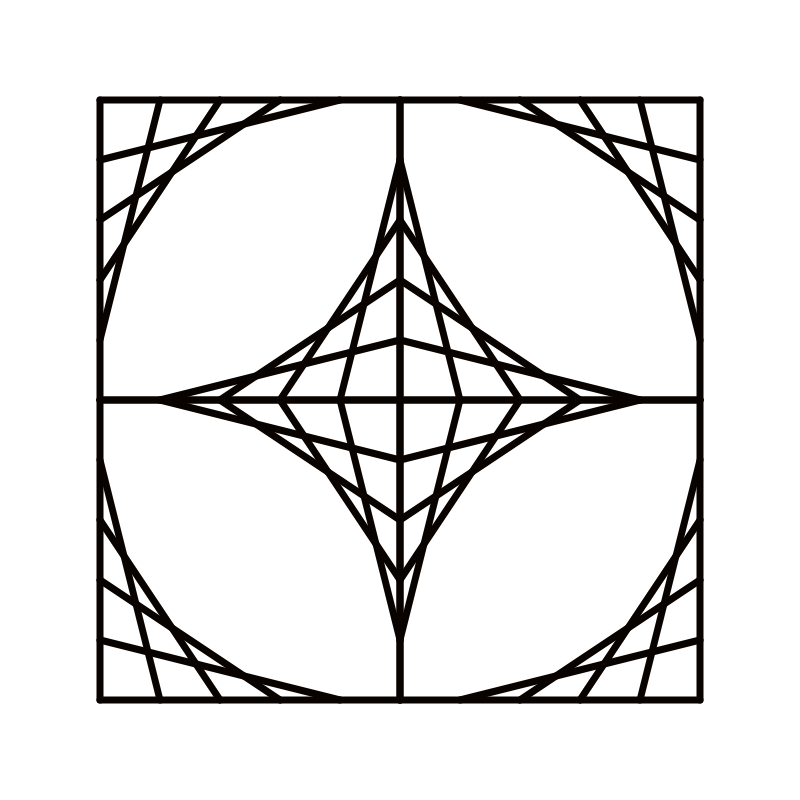
\includegraphics[width=.6\textwidth]{etD4.png}
 \end{center}
   Color this picture so that the only symmetries it has are:
   \begin{itemize}
   \item $e$ the do-nothing symmetry,
   \item $r$, a $180$ degree rotation, 
   \item $f$ a flip across a vertical line through the center, and
   \item $rf$ a flip across a horizontal line through the center.
   \end{itemize}
   \begin{freeResponse}
   Here's my picture:
   \begin{center}
     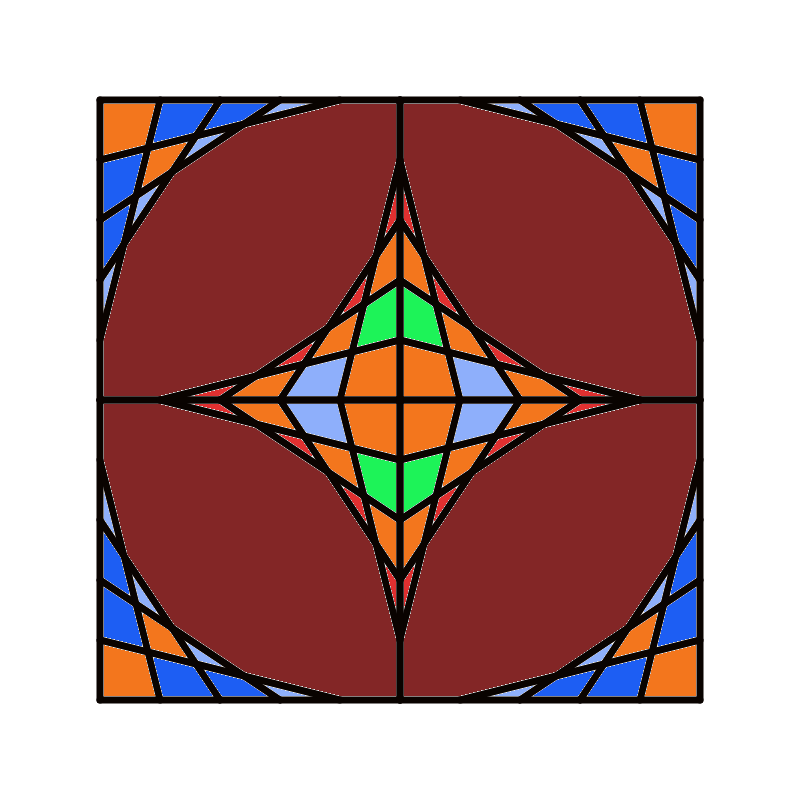
\includegraphics[width=.6\textwidth]{ciD4.png}
   \end{center}
 \end{freeResponse}

\end{question}
\mynewpage

\begin{question}
  Let $r$ represent a $90$ degree clockwise rotation and $f$
  represent a flip across a vertical line through the center of the
  picture.  
 \begin{enumerate}
 \item Use an envelope of tangents to draw a picture whose symmetries
   are $e,r,r^2,r^3,f,rf,r^2f$, $r^3f$.
 \item Now color-in your picture so that the only symmetries remaining
   are $e,r,r^2,r^3$.
 \end{enumerate}
\end{question}
\mynewpage



\begin{question}
  Let $r$ represent a $120$ degree clockwise rotation and $f$
  represent a flip across a vertical line through the center of the
  picture.  
 \begin{enumerate}
 \item Use an envelope of tangents to draw a picture whose symmetries
   are $e,r,r^2,f,rf,r^2f$.
 \item Now color-in your picture so that the only symmetries remaining
   are $e,r,r^2$.
 \end{enumerate}
 \begin{freeResponse}
   DUPLICATE
 \end{freeResponse}
\end{question}
\mynewpage


\begin{question}
  Let $r$ represent a $90$ degree clockwise rotation and $f$
  represent a flip across a vertical line through the center of the
  picture.  
 \begin{enumerate}
 \item Use an envelope of tangents to draw a picture whose symmetries
   are $e,r,r^2,r^3,f,rf,r^2f$, $r^3f$.
 \item Now change the number of LINES in your picture so that the only
   symmetries remaining are $e,r^2$.
 \end{enumerate}
 \begin{freeResponse}
 \begin{enumerate}  
 \item Here is my first drawing:
   \begin{center}
     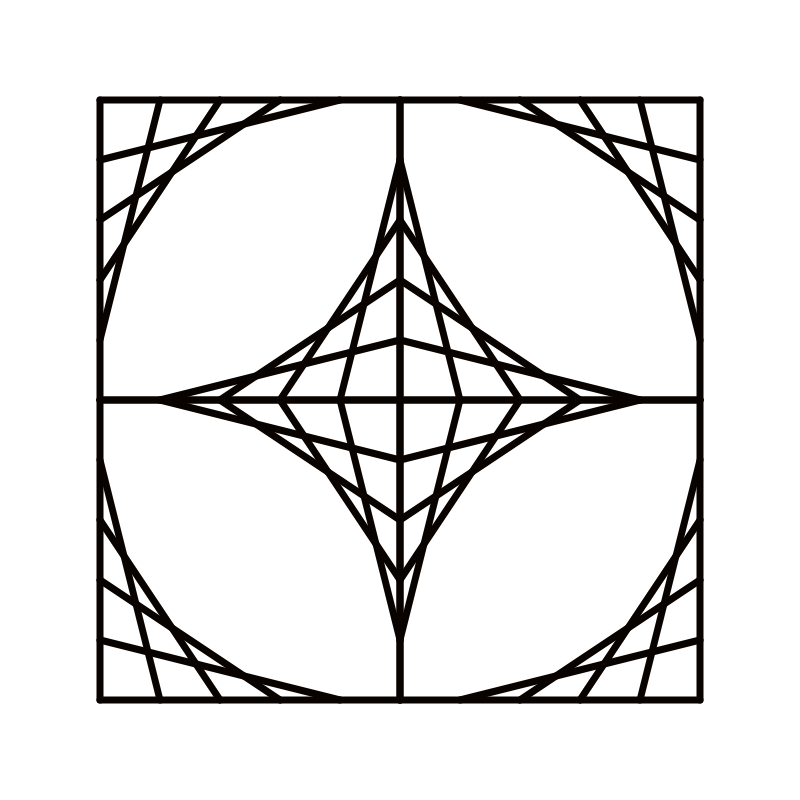
\includegraphics[width=.6\textwidth]{etD4.png}
   \end{center}
 \item Now colored in we have:
    \begin{center}
     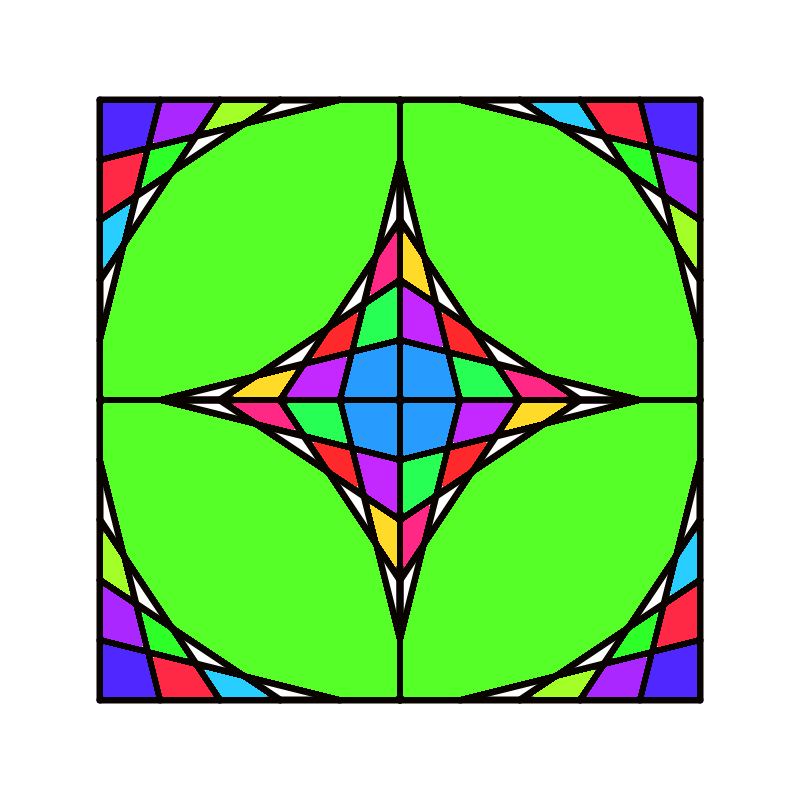
\includegraphics[width=.6\textwidth]{ciR4.png}
    \end{center}
 \end{enumerate}
 \end{freeResponse}
\end{question}
\mynewpage

\begin{question}
  This question is about symmetries of the equilateral triangle.
  \begin{enumerate}
  \item Let $f$, $g$, and $h$, be the symmetries of the equilateral
    triangle that are ``flips.''
    \begin{itemize}
    \item $f$ flips across a vertical line through the center of the triangle.
    \item $g$ flips across a line of positive slope.
    \item $h$ flips across a line of negative slope.
    \end{itemize}
    Express every symmetry of the equilateral triangle in terms of:
    \[
    e,f,g,h,fg,fh
    \]
  \item Make a MULTIPLICATION table for these elements. As a gesture
    of friendship, I have started this for you:
           \[
  \begin{array}{|c||c|c|c|c|c|c|}
    \hline
    & e & f & g & h & fg & fh\\ \hline\hline
    e &  &   &     &   &    &     \\ \hline
    f &   &     &   &    &      &  \\ \hline
    g &     &   &   &      &   &  \\ \hline
    h  &   &      &    &   &     &  \\ \hline
    fg &    &   &      &   &   &    \\ \hline
    fh &      &    &   &     &   &  \\ \hline
  \end{array}
  \]
  \item Let $r$ represent a $120$ degree clockwise rotation and $f$
    represent a flip across a vertical line through the center of the
    picture. CAN you draw a picture whose symmetries are
    \[
    e,r,r^2,f,rf,r^2f
    \]
    BUT when you color it some special way, it only has symmetries:
    \[
    e,f,rf,r^2f?
    \]
    WHY OR WHY NOT? EXPLAIN YOUR REASONING.
  \end{enumerate}
  \begin{freeResponse}
    \begin{enumerate}
    \item Here are the elements:
      \[
      e = e, r = fg, r^2 = fh, f= f, rf = h, r^2f=g.
      \]
    \item  Here's the table:
      \[
      \begin{array}{|c||c|c|c|c|c|c|}
        \hline
        & e  & f   & g  & h  & fg & fh  \\ \hline\hline
        e  & e  & f   & g  & h  & fg & fh  \\ \hline
        f  & f  & e   & fg & fh & g  & h   \\ \hline
        g  & g  & fh  & e  & fg & h  & f   \\ \hline
        h  & h  & fg  & fh & e  & f  & g   \\ \hline
        fg & fg & h   & f  & g  & fh & e   \\ \hline
        fh & fh & g   & h  & f  & e  & fg  \\ \hline
      \end{array}
      \]
    \item NO this is not possible. As soon as the object has
      symmetries through $f$, $g$, and $h$, it will have symmetries
      through $f^2$, $fg$ and $fh$, and these are the symmetries
      $e,r,r^2$.
    \end{enumerate}
  \end{freeResponse}
\end{question}


\end{document}
